%CLASSE DOCUMENTO - LINGUA E DIMENSIONE FONT
\documentclass[trieste,corpo=11pt,numerazioneromana]{toptesi}

%%%%%%%%%%%%%%%%%%%%%%%%%%%%%%%%%%%%%%%%%%%%%%%%%%%%%%%%%%%%%%%

% INCLUSIONE PACCHETTI
\usepackage[classica]{topfront}
\usepackage[utf8]{inputenc} %utf8
\usepackage[italian]{babel}
\usepackage[T1]{fontenc}
\usepackage{blindtext}
\usepackage{graphicx,wrapfig}
\usepackage{booktabs}
\usepackage{lmodern}
\usepackage{varioref}
\usepackage{epigraph}
\usepackage{url}
\usepackage{array}
\usepackage{paralist}{\obeyspaces\global\let =\space}
\usepackage{verbatim}
\usepackage{subfig}
\usepackage{tabularx}
\usepackage{amsmath}
\usepackage{amsfonts}
\usepackage{float}
\usepackage{float}
\usepackage{amssymb}
\usepackage{multicol}
\usepackage{multirow}
\usepackage{tabularx}
\usepackage{listings}
\usepackage[pass]{geometry}
\usepackage[figuresright]{rotating}
\usepackage{algorithm}
\usepackage{algorithmic}
\usepackage{wrapfig}
\usepackage{amsmath}
\usepackage[babel]{csquotes}
\usepackage{hyperref}
\usepackage{minted}
\usepackage[backend=biber,bibencoding=ascii]{biblatex}

%%%%%%%%%%%%%%%%%%%%%%%%%%%%%%%%%%%%%%%%%%%%%%%%%%%%%%%%%%%%%%%

% CONFIGURAZIONE LINK E RIFERIMENTI
\hypersetup{%
    pdfpagemode={UseOutlines},
    bookmarksopen,
    pdfstartview={FitH},
    colorlinks,
    linkcolor={black}, %COLORE DEI RIFERIMENTI AL TESTO
    citecolor={blue}, %COLORE DEI RIFERIMENTI ALLE CITAZIONI
    urlcolor={blue} %COLORI DEGLI URL
}

%%%%%%%%%%%%%%%%%%%%%%%%%%%%%%%%%%%%%%%%%%%%%%%%%%%%%%%%%%%%%%%

% CONFIGURAZIONE LISTATI/CODICE - CANCELLARE SE NON NECESSARIO
% PYTHON - BIANCO E NERO
\lstset{%
	captionpos=b,
	language=Python,
	basicstyle =\small\ttfamily,
	keywordstyle=\color{black}\bfseries,
	breaklines=true,
	breakatwhitespace=true,
	frame=lines,
	numbers=left,
	numberstyle=\footnotesize,
}

%%%%%%%%%%%%%%%%%%%%%%%%%%%%%%%%%%%%%%%%%%%%%%%%%%%%%%%%%%%%%%%

% FRENCHSPACING VA _SEMPRE_ ABILITATO PER DOCUMENTI IN ITALIANO
\frenchspacing

%%%%%%%%%%%%%%%%%%%%%%%%%%%%%%%%%%%%%%%%%%%%%%%%%%%%%%%%%%%%%%%

%DEFINIZIONE SEZIONI IN NUMERAZIONE ROMANA
%ELENCO DEI LISTATI/CODICI
\makeatletter
\newcommand\listofcodes{%
 \iffrontmatter\else\frontmattertrue\fi
 \if@openright\cleardoublepage\else\clearpage\fi
 % change the meaning of \chapter in a group
 \begingroup\def\chapter##1{\@schapter}
 \phantomsection % for the hyperlink
 \addcontentsline{toc}{chapter}{Elenco dei listati}
 \lstlistoflistings
 \endgroup
}
\makeatother

\addto\captionsitalian{%
  \renewcommand{\lstlistlistingname}{Elenco dei listati}%
  \renewcommand{\lstlistingname}{Listato}%
}

%%%%%%%%%%%%%%%%%%%%%%%%%%%%%%%%%%%%%%%%%%%%%%%%%%%%%%%%%%%%%%%

% INFORMAZIONI PDF - PERSONALIZZARE
\pdfinfo{%
  /Title    (Realizzazione di un assistente vocale per il triage ospedaliero)
  /Author   (Simone Montali)
  /Subject  (Triage semi-automatizzato per la sicurezza e la tempestività)
  /Keywords (Triage ML Mycroft Ospedale Hospital)
}

%%%%%%%%%%%%%%%%%%%%%%%%%%%%%%%%%%%%%%%%%%%%%%%%%%%%%%%%%%%%%%%

% LISTA DEI CAPITOLI DA INCLUDERE - PERSONALIZZARE
\includeonly{%
introduzione,%
stateofart,%
mycroft,%
skills,%
inference,%
app_a,%
}

% FILE DI BIBLIOGRAFIA
\addbibresource{bibliography.bib}

%%%%%%%%%%%%%%%%%%%%%%%%%%%%%%%%%%%%%%%%%%%%%%%%%%%%%%%%%%%%%%%

% INIZIO DOCUMENTO
\begin{document}

%%%%%%%%%%%%%%%%%%%%%%%%%%%%%%%%%%%%%%%%%%%%%%%%%%%%%%%%%%%%%%%

% FRONTESPIZIO - PERSONALIZZARE
% ELIMINATE LE VOCI CHE NON VI SERVONO

% UNIVERSITA - NOME
\ateneo{Università degli studi di Parma}

% FACOLTA - DICITURA - CANCELLARE O DECOMMENTARE
%\FacoltaDi{Faculty of}
% FACOLTA - NOME
\facolta{Ingegneria}

% CORSO DI LAUREA - DICITURA (MANTENERE LO SPAZIO) - CANCELLARE O DECOMMENTARE
%\CorsoDiLaureaIn{Master of Science in }
% CORSO DI LAUREA - NOME
\corsodilaurea{Ingegneria dei Sistemi Informativi}

% TIPOLOGIA TESI
\TesiDiLaurea{Tesi di Laurea di primo livello}

% TITOLO
\titolo{Realizzazione di un assistente vocale per il triage ospedaliero}

% SOTTOTITOLO
\sottotitolo{Triage semi-automatizzato per la sicurezza e la tempestività}

% RELATORE/I - DICITURA - CANCELLARE SE UN SOLO RELATORE
\AdvisorName{Relatori}
% RELATORE - PROF. NOME E COGNOME
\relatore{prof.ssa\ Mordonini Monica}
% RELATORE AGGIUNTIVO - PROF NOME E COGNOME
% SE SI HA SOLO UN RELATORE ELIMINARE INSIEME AD AdvisorName
\terzorelatore{prof.\ Tomaiuolo Michele}
%\terzorelatore{prof.\ Angiani Giulio}
% CANDIDATO - DICITURA (MANTENERE I DUE PUNTI) - CANCELLARE O DECOMMENTARE
%\CandidateName{Candidate:}

% CANDIDATO - NOME E COGNOME
\candidato{Simone Montali}[288144]

% LOGO UNIVERSITA
\logosede{images/logo}

% DATA - MESE ANNO
\sedutadilaurea{Probabilmente 2020}

\frontespizio

%%%%%%%%%%%%%%%%%%%%%%%%%%%%%%%%%%%%%%%%%%%%%%%%%%%%%%%%%%%%%%%

%INTERLINEA - DEFAULT 1 - NON ESAGERATE, NON SUPERATE MAI 1.3 ;)
%\interlinea{1.2}

%%%%%%%%%%%%%%%%%%%%%%%%%%%%%%%%%%%%%%%%%%%%%%%%%%%%%%%%%%%%%%%

\frontmatter

% DEDICA - PERSONALIZZARE
% VSPACE - PROPORZIONE USATA PER CENTRATURA VERTICALE DEL TESTO
% FLUSHRIGHT - ALLINEAMENTO ORIZZONTALE A DESTRA
\vspace*{\stretch{1}}
\begin{flushright}
  \noindent
  Dedica toccante.
\end{flushright}
\vspace*{\stretch{6}}
\cleardoublepage


% CITAZIONE - PERSONALIZZARE
% VSPACE - PROPORZIONE USATA PER CENTRATURA VERTICALE DEL TESTO
% FLUSHRIGHT - ALLINEAMENTO ORIZZONTALE A DESTRA
\vspace*{\stretch{1}}
\begin{flushright}
  \noindent
  Citatemi dicendo che sono stato citato male.

  \textit{Groucho Marx}
\end{flushright}
\vspace*{\stretch{6}}
\cleardoublepage

%%%%%%%%%%%%%%%%%%%%%%%%%%%%%%%%%%%%%%%%%%%%%%%%%%%%%%%%%%%%%%%

% RINGRAZIAMENTI - PERSONALIZZARE
\ringraziamenti
Grazie

%%%%%%%%%%%%%%%%%%%%%%%%%%%%%%%%%%%%%%%%%%%%%%%%%%%%%%%%%%%%%%%

% ABSTRACT - PERSONALIZZARE
\sommario
Abstract della tesi
%%%%%%%%%%%%%%%%%%%%%%%%%%%%%%%%%%%%%%%%%%%%%%%%%%%%%%%%%%%%%%%

% INDICI - ELIMINARE GLI INDICI NON NECESSARI

% INDICE GENERALE
\tableofcontents

% INDICE DELLE FIGURE
\listoffigures

% INDICE DELLE TABELLE
%\listoftables

% INDICE DEI CODICI
%\listofcodes

%%%%%%%%%%%%%%%%%%%%%%%%%%%%%%%%%%%%%%%%%%%%%%%%%%%%%%%%%%%%%%%

\mainmatter

% INCLUSIONE FILE CAPITOLI - PERSONALIZZARE - TENERE COERENTE CON LISTA IN ALTO
\chapter{Introduzione}
\label{chap:introduzione}
In una società sempre più digitalizzata e dinamica, spesso viene a crearsi un netto distacco tra i settori capaci di \textbf{evolvere assieme alla tecnologia}, e quelli che, per un motivo o per l'altro, rimangono ancorati a procedure e metodologie tradizionali. Il settore medico, in continuo rinnovamento sul lato scientifico, è, soprattutto in Italia, affidato ad \textbf{infrastrutture informatiche progettate tempo fa.} Questo, soprattutto per motivi di stabilità e affidabilità: gli errori, qui, non sono ammissibili. \\
Per questo motivo, spesso non si notano le evidenti possibilità di miglioramenti che la ricerca informatica potrebbe apportare agli ospedali, agli ambulatori, agli studi.
L'obiettivo di questa tesi è mettere luce su una delle possibili modalità con cui l'informatica potrebbe, in un futuro prossimo, migliorare la praticità ma soprattutto la sicurezza degli ambienti ospedalieri.\\
La procedura di triage, ossia il processo di selezione dei pazienti richiedenti cure, è oggi affidata totalmente ad infermieri. Questa scelta è dovuta, oltre ad un evidente bisogno di poter osservare il paziente, alla necessità dell'\textbf{immediatezza di un contatto verbale} con il personale sanitario. \\
Perciò, la sfida nella realizzazione della tesi è soprattutto legata al rendere il \textbf{più umana possibile} l'interazione con un bot automatizzato. Il bot deve quindi accogliere il paziente, comprenderne le problematiche ed i sintomi, e farlo sentire protetto. Non si escluderà del tutto un apporto umano: gli infermieri sono addestrati per poter osservare e comprendere il richiedente cura, e l'apporto dell'osservazione diretta del paziente è ancora troppo importante per escluderla. È senz'altro possibile, però, affidare la prima parte di \textbf{profilazione dell'utente} a procedure automatizzate.

\chapter{Stato dell'arte}
\label{chap:stateofart}
Impara l'arte e mettila da parte.

\chapter{Mycroft}
\label{chap:mycroft}
\epigraph{There’s an entire community of developers looking to access this technology, but so far, it’s been the purview of a few large companies. The technology is walled-off, proprietary, and secretive.}{\textit{Joshua Montgomery \\ CEO di Mycroft AI, Inc.}}
Nel panorama degli assistenti vocali disponibili al pubblico, le grandi aziende catturano la maggior parte delle attenzioni dei consumatori. I nomi di Amazon Alexa, Google Home, Microsoft Cortana sono familiari a tanti. Meno familiare, però, è lo scenario degli stessi strumenti in ambito di assistenti vocali. Piattaforme come \textit{Jarvis}, \textit{Linto}, \textit{Open Assistant} e \textbf{Mycroft} sono sconosciute ai più. Quest'ultimo, negli ultimi anni, ha catturato l'attenzione di molti esperti di settore per la sua stabilità, espansibilità, popolarità.
\section{Open source}
\subsection{Cosa si intende con open source?}
Il termine \textbf{open source} si riferisce a qualcosa di modificabile e condivisibile dalle persone, avente quindi un \textbf{design pubblicamente accessibile.} Il termine nacque nell'ambito dello sviluppo software, ma oggi rappresenta, piuttosto, un'etica. Il software open source è software il cui codice sorgente è ispezionabile, modificabile, e migliorabile da chiunque voglia farlo. Con \textit{codice sorgente} intendiamo il codice che definisce il comportamento del programma, ossia il prodotto del lavoro di un programmatore. \\
Molti dei software che oggi utilizziamo sono invece \textbf{closed source} (o \textit{proprietario}), ossia software il cui codice sorgente non è accessibile agli utenti, e sul quale l'organizzazione che crea il software ha \textit{pieni poteri}. Alcuni esempi di software proprietario possono essere Windows, Photoshop, Safari. Solitamente, durante l'installazione di uno di questi software, l'utente accetta dei termini e condizioni che lo vincolano a non fare nulla di non autorizzato dall'azienda creatrice del software.
\subsection{Perché open source?}
Le motivazioni per preferire software open source rispetto a quelli proprietari sono svariate. Sebbene i software proprietari spesso abbiano funzionalità più avanzate e, spesso, meglio sviluppate, hanno gravi mancanze in progetti come questo. Il software open source, a scapito della possibilità di minori funzionalità (nonostante ciò non sia sempre vero, basti pensare alla potenza del kernel Linux), dà ad un utente esperto tante possibilità:
\begin{itemize}
    \item Possibilità di \textbf{controllo} sul software: la modifica e il miglioramento del software è permessa e ben vista. La comunità open source lavora con coesione per produrre software sempre migliore.
    \item Possibilità di conoscere e studiare i \textbf{meccanismi interni}: l'utilizzo di software per fini scientifici richiede la piena conoscenza di come un software funziona. Inoltre, la disponibilità del codice a tutti permette agli studenti e agli interessati di scoprire le logiche che ne permettono il corretto funzionamento.
    \item Grandi garanzie di \textbf{sicurezza}: se tutti possono accedere al codice, la presenza di bug di sicurezza e problematiche di privacy viene rilevata molto più velocemente di come accade nel software proprietario.
    \item Certezze sulla \textbf{privacy}: la società in cui viviamo è sempre più basata sulla vendita di dati personali acquisiti tramite software. L'open source, spesso e volentieri, si oppone a tale tendenza: essendo software della comunità e non di un'azienda che punta all'ottenimento di capitale, nessuno ha interesse nel \textit{monetizzare gli utenti}.
    \item Supporto della \textbf{comunità}: lo sviluppo di software open source è molto supportato dalla comunità informatica. In caso di problematiche o necessità, ci sarà sempre un utente più esperto disposto ad aiutare.
    \item Correttezza \textbf{etica}: software come quello oggetto di questa tesi hanno l'obiettivo di salvare vite. È giusto che tutti possano accedervi, migliorarlo e conoscerlo. La ricerca scientifica dovrebbe essere il più possibile \textbf{libera}.
\end{itemize}
\section{Introduzione a Mycroft}
Mycroft nacque tramite crowdfunding nel 2015 e catturò subito molto interesse da parte della comunità informatica. L'obiettivo era chiaro: opporsi alla sola presenza di software proprietario nel campo degli assistenti vocali. Ricevette presto l'appoggio di molte organizzazioni come la Canonical (promotrice di Ubuntu) e la Mozilla Foundation. La repository su Github di Mycroft conta oggi \textit{4300 stars} in continua crescita.
\subsection{Stack di funzionamento}
Come spiegato nel capitolo \ref{section:vocal_assistants}, un assistente vocale si compone principalmente di:
\subsubsection{Rilevamento della wake word}
L'assistente ha bisogno di rilevare una parola per attivarsi. Gli esempi più famosi sono \textit{Hey, Google} o \textit{Alexa}. Mycroft permette di personalizzare la propria wake word, che all'installazione è semplicemente \textit{Hey, Mycroft}. Il progetto utilizza \textbf{Precise}, un wake word listener basato su reti neurali addestrate su esempi audio. Questo componente, totalmente open source, è basato su \textit{pattern sonori}, non sul testo. La caratteristica ne riduce la dipendenza da accenti e linguaggi diversi. Precise offre la possibilità di addestrare il listener su un proprio dataset. Il funzionamento è basato su una singola rete neurale ricorrente, più precisamente una \textbf{Gated Recurrent Unit} o GRU.
\begin{figure}[H]
    \begin{center}
        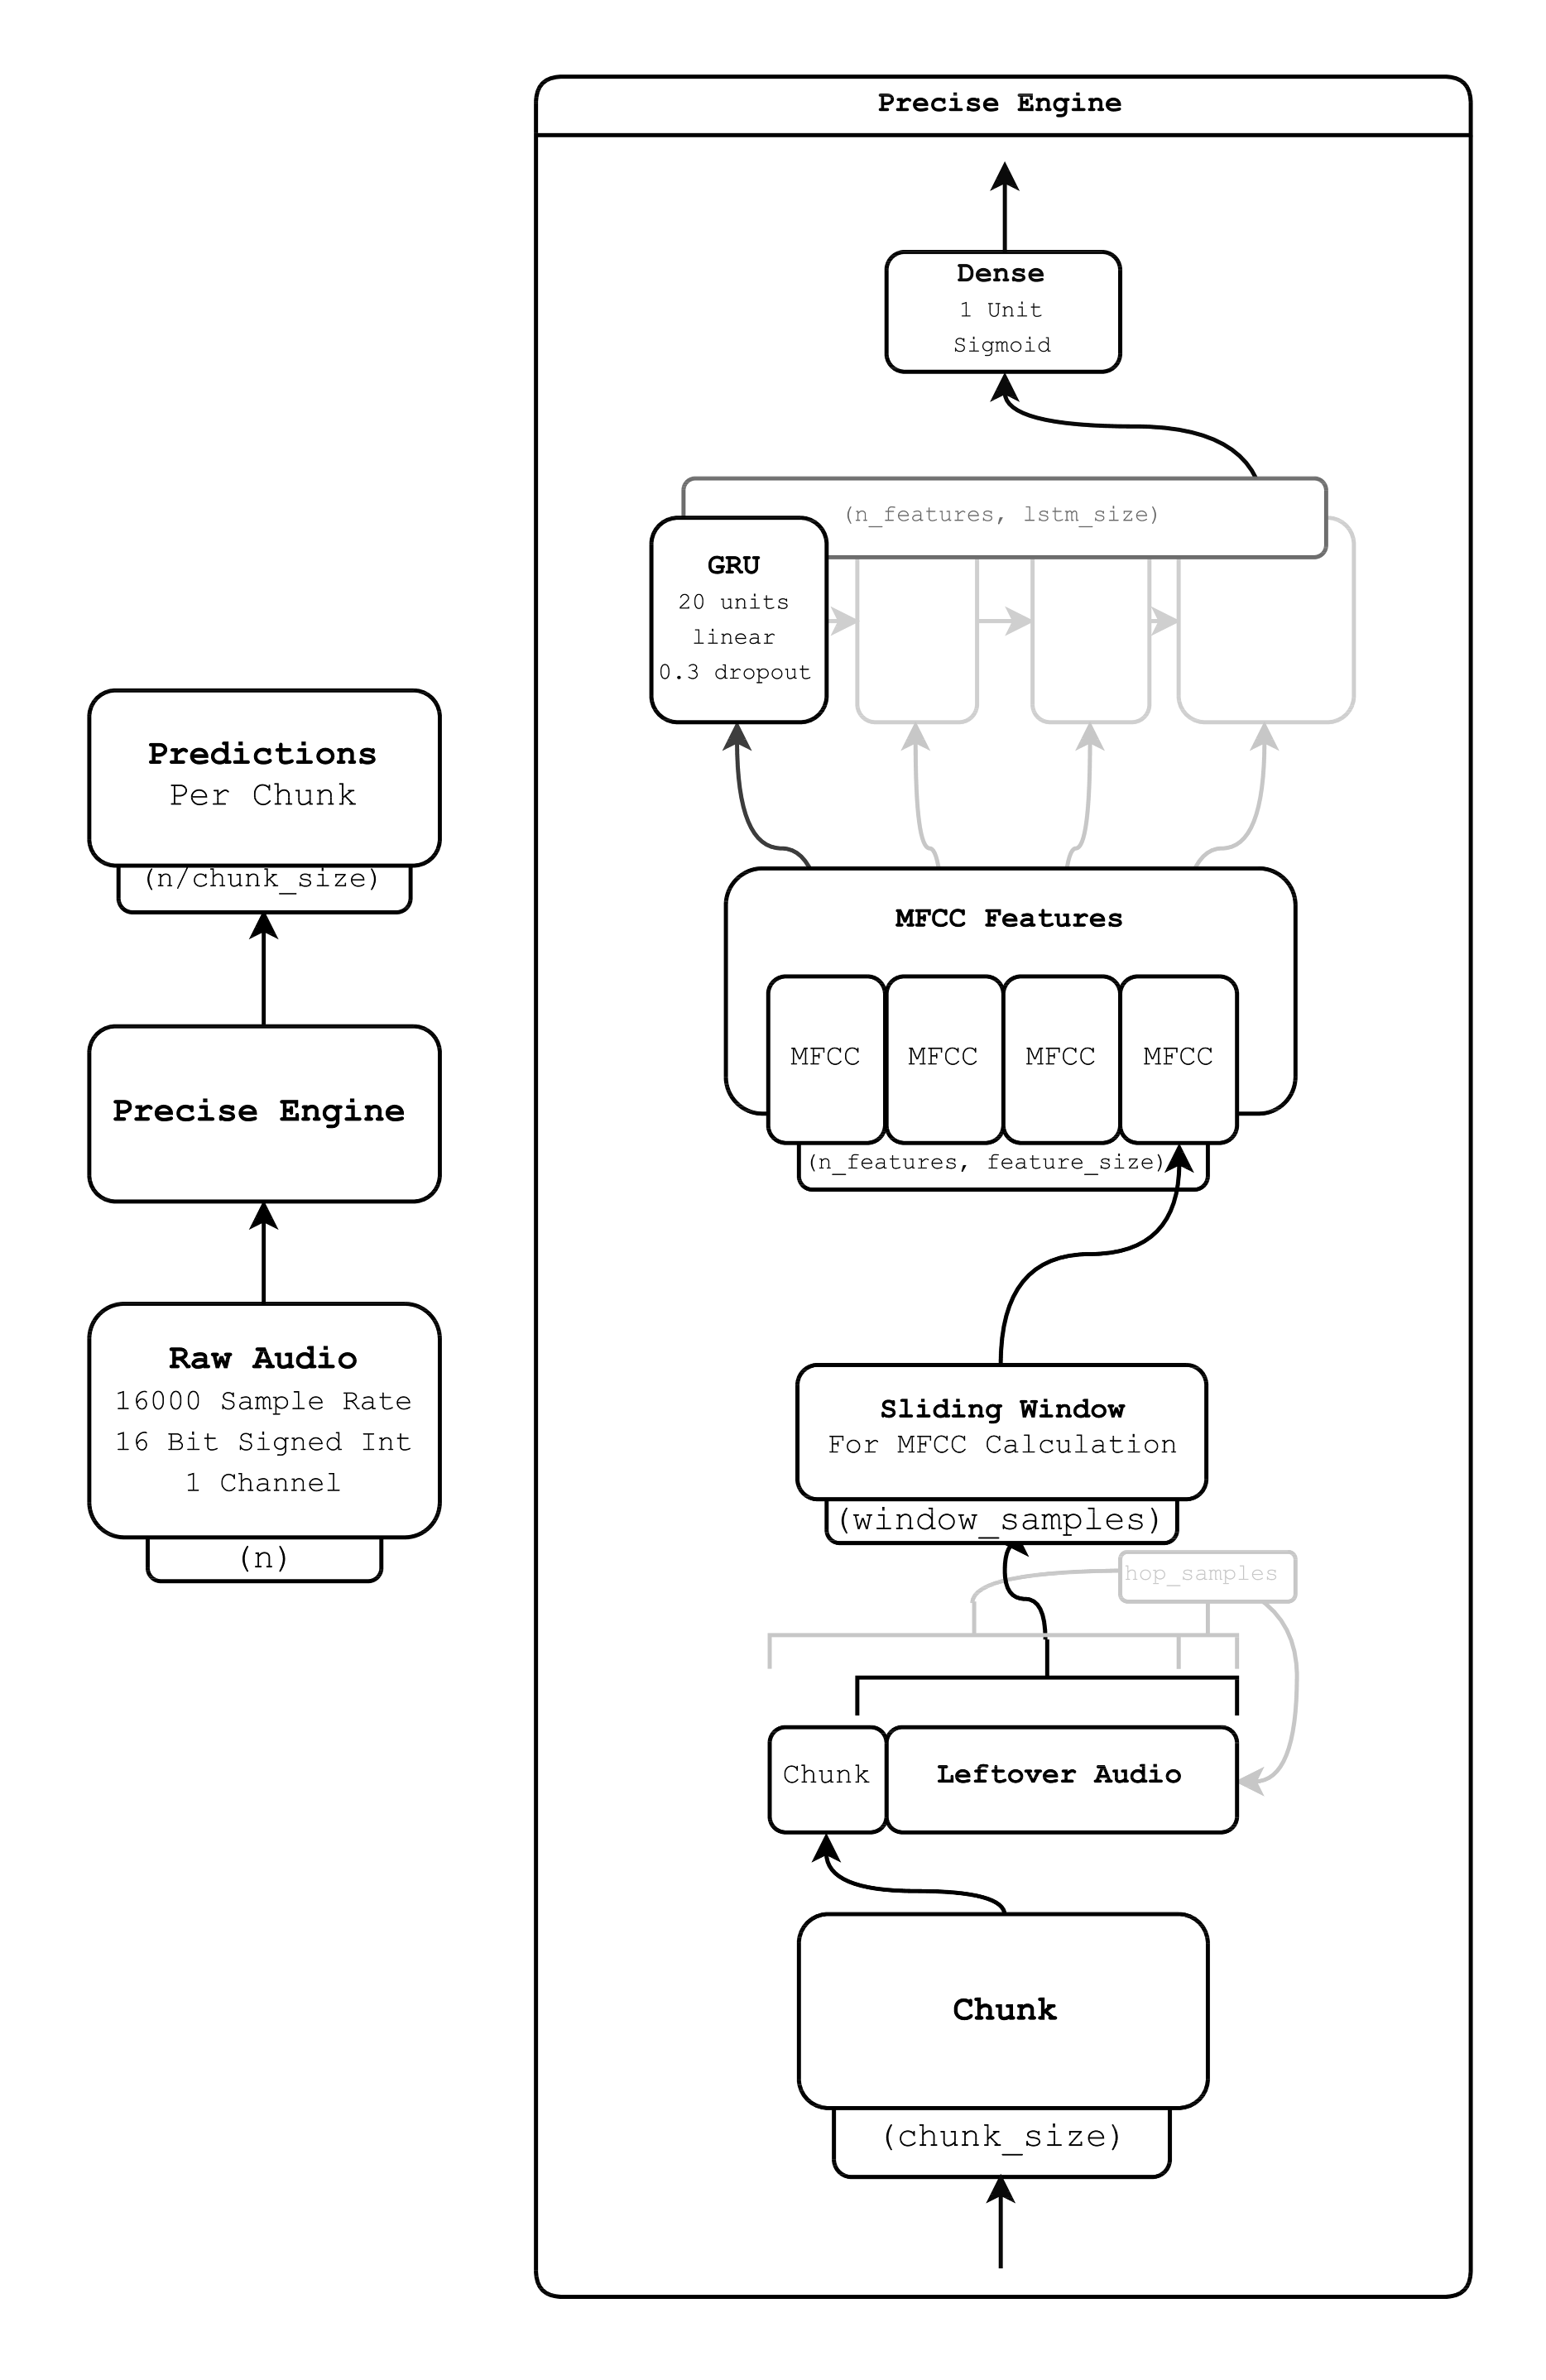
\includegraphics[width=0.6\columnwidth]{images/mycroft/precise.png}
    \end{center}
    \caption{Schema di funzionamento di Precise}
    \label{fig:precise}
\end{figure}
\subsubsection{Speech To Text}
Mycroft sfrutta il motore STT di Google per effettuare questo processo. Per aggiungere uno strato di privacy a queste richieste, esse vengono fatte passare attraverso i server Mycroft: Google non può ricollegare una richiesta all'utente che l'ha fatta. In questo modo, tutte le query effettuate a Google contengono solamente l'audio e hanno lo stesso mittente. In futuro sarà possibile sfruttare il dataset di \textbf{Mozilla Deepspeech}, che non è, ad oggi, ancora sufficientemente affidabile.
\subsubsection{Interpretazione degli intent}
Nell'ambito della speech recognition, un intent è l'operazione che l'utente \textit{intende} svolgere. Un utente può richiedere un'operazione in modi molto diversi. Lo scopo dell'intent parser è proprio quello di riuscire a superare questo scoglio, estraendo dalla richiesta scritta gli elementi chiave. Per esempio, se avessimo una richiesta del tipo "Hey Mycroft, domani pioverà a Parma?", l'intent parser dovrebbe capire:
\begin{itemize}
    \item L'utente desidera conoscere il \textbf{tempo atmosferico}.
    \item Il tempo atmosferico deve essere cercato per \textbf{Parma}.
    \item La data di interesse è \textbf{domani}.
\end{itemize}
Mycroft rende disponibili due software per la rilevazione di intenti: Padatious e Adapt. Mentre il secondo è basato sul riconoscimento di parole chiave, ed è quindi molto suscettibile alle richieste, il primo è composto da una rete neurale addestrata su frasi intere. Nel corso del progetto sfrutteremo \textbf{Padatious}.
Questo motore permette di avere creazione semplice degli intent, quantità di dati relativamente bassa, estrazione delle \textit{entities} semplice, addestramento rapido.
\subsubsection{Text To Speech}
Il componente di Text To Speech ha il compito di generare una traccia audio partendo dal testo di risposta codificato nella skill. Mycroft rende disponibile il progetto \textbf{Mimic}, basato sul software FLITE dell'università Carnegie Mellon. Purtroppo quest'ultimo non è disponibile in italiano, quindi nel corso del progetto utilizzeremo il motore TTS di Google, ottimizzato per l'italiano. Come sempre, le richieste passano attraverso i server Mycroft per ottenere un buon livello di privacy.
I testi di risposta sono codificati nei file vocabolario delle skills.
\subsection{Interfaccia grafica}
I dispositivi più avanzati di Mycroft come il \textit{Mark II} forniscono la possibilità di aggiungere interazioni visive con gli utenti. L'interfaccia è gestita da Mycroft-GUI, un componente aggiuntivo del bot che sfrutta i KDE Plasmoids, oggetti dell'interfaccia grafica KDE Plasma, simili a widget. La tecnologia è basata sul linguaggio QML, che permette una totale libertà nella creazione di interfacce, ma anche dei template standard semplici e rapidi da implementare. QML fa parte dello stack di tecnologie di Qt, una libreria multipiattaforma per lo sviluppo di programmi con interfaccia grafica.
\chapter{Realizzazione di skills}
\label{chap:skills}
Mycroft permette di espandere le abilità del bot in maniera semplice: è infatti costruito modularmente, ed è in ogni momento possibile espandere o ridurre i moduli attivi.
Questi moduli sono detti \textbf{skills}. Ogni skill è responsabile di una funzionalità: avremo ad esempio la skill del meteo, la skill che racconta barzellette o la skill che si occupa della domotica. Alla ricezione di una richiesta, Mycroft verifica gli intent e le keywords di ogni skill, attivando quella giusta.
% TODO: flowchart con adapt+padatious
La creazione di nuove skills è possibile grazie alla classe Python \texttt{MycroftSkill}, tramite la cui espansione possiamo definire i comportamenti della skill. All'installazione di Mycroft verrà reso disponibile il \textbf{Mycroft Skills Kit}, una command line interface che permette di eseguire le operazioni fondamentali collegate alle skills Mycroft. Tramite il comando \texttt{mycroft-msk create} verrà avviata una CLI che, dopo aver richiesto al programmatore alcune informazioni, genera il \textit{boilerplate code} necessario alla realizzazione della skill. Tra le informazioni richieste avremo nome, frasi d'esempio, dialoghi di risposta, descrizioni, etc\dots
Il template viene inoltre fornito di \texttt{git}, un sistema di versioning che permette di tenere traccia delle modifiche al codice e semplificare l'interazione tra programmatori.
\section{Struttura dei file della skill}
La struttura delle skills è ben organizzata, e vi sono diverse tipologie di file. Oltre a licenza e README, abbiamo tre componenti fondamentali per il funzionamento.
% TODO: dirtree
\paragraph{Directory \texttt{locale}}
Questa directory contiene i file dipendenti dalla lingua. Le sottocartelle seguono i tag linguistici IETF, quindi l'italiano sarà rappresentato da \texttt{it-it} e l'inglese (americano) da \texttt{en-us}. All'interno di queste, possiamo incontrare quattro tipologie di file:
\begin{itemize}
    \item \textbf{\texttt{dialog}}: questi file contengono i dialoghi di risposta del bot. Sono presenti più frasi simili, in modo da avere interazioni più "umane" con il bot, che sceglie una frase casuale tra queste. Ad esempio, \texttt{get\_age.dialog} conterrà le frasi \textit{"Mi potresti dire quanti anni hai?"}, \textit{"Per favore, dimmi la tua età"}, \textit{"Qual è la tua età?"}...
    \item \textbf{\texttt{intent}}: questi file contengono le frasi utilizzate per addestrare la rete neurale di Padatious. Ovviamente, più esempi vengono fatti, meglio la rete funzionerà. Per esempio, il file \texttt{symptoms.bleeding.intent} conterrà frasi come \textit{"Ho un'emorragia"}, \textit{"Sto sanguinando molto"}, \textit{"Ho una grande perdita di sangue"}...
    \item \textbf{\texttt{voc}}: questi file contengono keywords utilizzate in Adapt e nelle domande a risposta chiusa. Siccome il progetto si basa fortemente su Padatious, troviamo solo i file vocabolario per le domande sì/no ed il riconoscimento di numeri. Ad esempio, il file \texttt{yes.voc} conterrà \textit{"Sì"}, \textit{"Certo"}, \textit{"Esatto"}...
    \item \textbf{\texttt{entity}}: questi file contengono entità da estrarre negli intent. Ad esempio, l'intent \textit{fratture} estrae l'arto coinvolto nella frattura. Il file \texttt{limb.entity} conterrà quindi termini come \textit{"gamba"}, \textit{"pollice"}, \textit{"spalla"}...
\end{itemize}
\paragraph{\texttt{settingsmeta.yaml}}
Questo file contiene la definizione di impostazioni modificabili dall'utente sul sito di gestione di Mycroft. Ad esempio, l'utente potrebbe voler impostare i comportamenti di default, il nome del file esportato dal bot, una chiave API per l'integrazione con altri tool.
\paragraph{\texttt{\_\_init\_\_.py}}
Questo è il file principale della skill. Contiene il codice che definisce i comportamenti della skill. Il funzionamento è basato sull'espansione della classe \texttt{MycroftSkill}, che contiene i decorator ed i metodi necessari alla gestione della skill. Il prossimo capitolo si occuperà di definire la realizzazione vera e propria.
\section{Funzionamento della skill}
Tutta la realizzazione della skill è articolata intorno alla classe \texttt{MycroftSkill}.
\begin{minted}{python}
"""Mycroft skill that does a pre-triage on hospital patients.

The skill tries to ask the patient its symptoms, its personal data, 
and more. Then, it assigns a color code, stating a priority for
medical interventions.
"""

from mycroft import MycroftSkill, intent_file_handler
import json

class HospitalTriage(MycroftSkill):
    """Main skill class for the triage.

    This is the main skill class (extending MycroftSkill),
    which contains all the operations we need to perform the
    triage.

    Attributes:
        med_record: a dict containing all the patient data.
    """

    def __init__(self):
        MycroftSkill.__init__(self)
        self.med_record = {}
\end{minted}
\subsection{Metodi relativi alle sintomatologie}
La skill è stata strutturata come segue: ogni tipologia di sintomi equivale ad un intent, ed è quindi gestita da un metodo specifico. In base alla tipologia di sintomo, l'interazione viene poi gestita in modalità diverse: verrà assegnato al paziente un codice di triage, viene confermata al paziente la corretta comprensione del sintomo, viene mostrata sulla GUI l'informazione recepita. Terminate le operazioni specifiche del sintomo, le restanti procedure vengono gestite da decorators: la richiesta dell'anagrafica, dei sintomi minori, della febbre vengono eseguite indipendentemente dal problema riportato dal paziente. Un esempio di metodo relativo alle sintomatologie può essere il seguente:
\begin{minted}{python}
# BREATH
@intent_file_handler('symptoms.breath.intent')
@symptom_handler
@covid_symptom
def handle_breathing(self, message):
    """This function handles a "breathing fatigue" symptom.

    Breathing fatigue is recognized as a red code, and is a
    COVID-compatible symptom.

    Args:
        message: the message object returned from Mycroft

    GUI: show open mouth emoji
    """
    self.med_record["main_symptom"] = "breathing"
    self.med_record["code"] = "red"
    self.speak_dialog('symptoms.breath')
\end{minted}
Il metodo salva nell'oggetto \texttt{med\_record} (\textit{scheda clinica}) il sintomo principale, ossia problemi di respirazione, ed il codice relativo, in questo caso il rosso (accesso immediato alle cure). Poi, tramite il metodo \texttt{speak\_dialog} di \texttt{MycroftSkill}, pronuncia uno a caso tra i dialoghi contenuti nel file \texttt{symptoms.breath.dialog}, come
\begin{itemize}
    \item \textit{"Capisco, qualche problema di respirazione."}
    \item \textit{"Ok, segno nella scheda problemi di respirazione."}
    \item \textit{"Capito: problemi di respirazione."}
\end{itemize}
Da qui in poi, le operazioni sono affidate ai metodi chiamati dai decorators.
\subsection{Decorators utilizzati}
\subsubsection{Che cos'è un decorator?}
Anzitutto, occorre definire il comportamento di un decorator. Esso permette di assegnare responsabilità addizionali ad un oggetto, dinamicamente. Fornisce quindi un'alternativa flessibile al \textit{subclassing}. Definire un decorator in Python significa definire dei comportamenti da eseguire prima e dopo l'esecuzione del metodo vero e proprio.
\subsubsection{Applicazione del concetto al programma}
Alcune operazioni sono, all'interno del progetto, ricorrenti. Ad esempio, la richiesta di anagrafica o di sintomi minori deve essere fatta in tutti e soli i metodi relativi alla gestione di sintomi. Alcuni di questi (quelli compatibili con il COVID19, come la tosse), avranno bisogno inoltre di approfondimenti per valutare la possibilità che il paziente sia affetto da COVID19, facendogli domande specifiche. Sono stati quindi definiti due decorators aggiuntivi:
\paragraph{\texttt{symptom\_handler}} Questo metodo, dopo aver gestito le operazioni specifiche di un sintomo, prosegue con le procedure generali, come la richiesta dell'anagrafica, di una valutazione del dolore, di altri sintomi, e, per ultima, l'esportazione della cartella clinica.
\begin{minted}{python}
def symptom_handler(handler):
"""Decorates a symptom with the needed operations.

This function is used as a decorator for symptoms, adding
operations like personal data asking, age, other symptoms...

Returns:
    The decorator function
"""
def ask_about_symptoms(*args, **kwargs):
    returned = handler(*args, **kwargs)
    args[0].med_record["symptom_declaration"] = args[1].data["utterance"]
    # I'm using args[0] here instead of self, but it works the same
    args[0].request_age()
    args[0].request_other_symptoms()
    args[0].evaluate_pain()
    args[0].request_name()
    args[0].export_med_record()
    return returned
return ask_about_symptoms
\end{minted}
\paragraph{\texttt{covid\_symptom}} La situazione di emergenza che il mondo sta vivendo al momento della stesura di questa tesi ha richiesto particolare attenzione verso le sintomatologie compatibili con COVID19: distanziare i pazienti che potrebbero essere portatori di virus al più presto è la \textbf{sfida più grande del momento}. Per questo, il decorator, aggiunto ai soli sintomi compatibili con la malattia, permette di interrogare il paziente riguardo alcune caratteristiche tipiche della malattia, come il fiato corto, la difficoltà a percepire i sapori, la febbre alta.
\begin{minted}{python}
def covid_symptom(handler):
        """Decorates a COVID-compatible symptom.

        This function is used as a decorator in the COVID-compatible
        symptoms. It proceeds to ask the COVID-related questions
        to the patient.

        Returns:
            The decorator function
        """
        def check_if_covid(*args, **kwargs):
            returned = handler(*args, **kwargs)
            args[0].ask_covid_questions()
            return returned
        return check_if_covid
\end{minted}
Il metodo \texttt{ask\_covid\_questions} procede ad intervistare il paziente con il modello di diagnosi più usato al momento. Ogni domanda posta al paziente ha un suo \textit{score} caratteristico, che moltiplica un indice relativo al paziente in base alla gravità ed alla connessione con la malattia. Le caratteristiche indagate sono:
\begin{itemize}
    \item \textbf{Febbre}: moltiplicatore $2$
    \item \textbf{Mal di gola}: moltiplicatore $1.3$
    \item \textbf{Raffreddore}: moltiplicatore $1.3$
    \item \textbf{Fatica respiratoria}: moltiplicatore $1.6$
    \item \textbf{Tosse}: moltiplicatore $1.6$
    \item \textbf{Contatti con infetti}: moltiplicatore $2$
    \item \textbf{Mancanza di gusto}: moltiplicatore $1.7$
\end{itemize}
Ogni paziente sospetto ha inizialmente un \texttt{covid\_score} di $1$, che viene moltiplicato per i vari indici se il paziente risponde in modo affermativo. Se lo score supera una soglia predeterminata (al momento fissata a $15$), è sospetto COVID19 e verrà destinato ad un'area di triage apposita.
\begin{minted}{python}
def ask_covid_questions(self):
    """Checks for COVID symptoms.

    When triggered by a COVID-compatible symptom, 
    this function evaluates the patient symptoms to 
    try to guess if he/she has COVID19.

    GUI: show face mask emoji
    """
    self.speak_dialog('gotta_check_covid')
    covid_score = 1
    # Let's check if the patient knows the temperature. Skip if he already declared it.
    if not "fever" in self.med_record:
        self.check_fever()
    if "fever" in self.med_record:
        if self.med_record["fever"] > 37.5:
            covid_score = covid_score * 2
    # Let's define an array of tuples, each containing the yes/no question
    # string and its COVID index multiplier
    yesno_questions = [("has_sore_throat", 1.3), ("has_cold", 1.3),
     ("has_breathing_difficulties",1.6), ("has_cough", 1.6),
     ("has_had_contacts", 2), ("misses_taste", 1.7)]
    self.speak_dialog('will_ask_yesno')
    # Check if he/she has COVID-compatible symptoms
    for question in yesno_questions:
        self.med_record[question[0]] = self.ask_yesno(question[0])
        if self.med_record[question[0]] == 'yes':
            covid_score = covid_score * question[1]
        self.log.info(covid_score)

    self.med_record["covid_score"] = covid_score
    if covid_score > 15:
        self.speak_dialog('probably_has_covid')
    else:
        self.speak_dialog('doesnt_have_covid')
    self.log.info(self.med_record)
\end{minted}
\subsection{Helper methods}
Sono, oltre ai metodi caratteristici della classe, presenti alcuni \textit{helper methods} utili ad operazioni interne del software. Di seguito elenchiamo i più importanti:
\paragraph{\texttt{extract\_temperature}} Questo metodo, data una stringa in ingresso rappresentante la temperatura corporea che può essere in vari formati (ad esempio, il paziente potrebbe pronunciare \textit{"Trentasette e mezzo", "Trentasette virgola cinque", "Trentasette punto cinque", "Trentasette e cinque"} indicando sempre la stessa temperatura), la estrae in formato decimale.
\begin{minted}{python}
def extract_temperature(utterance):
    """Extracts the patient temperature from the utterance.

    This is needed because of the various ways of Mycroft interpreting
    floating point numbers. Some examples:
    - 38 e 1
    - 38/1
    - 38.1
    - 38,1
    - 38 1

    Returns:
        The floating point value of the temperature, or
        None if it is impossible to extract.
    """
    # Beware: the ' e ' has to be before the simple space!
    possible_separators = ['/', '.', ',', ' e ', ' ']
    try:
        for separator in possible_separators:
            if separator in utterance:
                temperature_strings = utterance.split(separator)
                if temperature_strings[1] == "mezzo":
                    temperature_strings[1] = "5"
                temperature = int(
                    temperature_strings[0])+float(temperature_strings[1])*0.1
                return temperature
        return None
    except TypeError:
        return None
\end{minted}
\paragraph{\texttt{age\_validator}} Questo metodo, fornito al metodo \texttt{get\_response}, definisce se un'età è valida. In caso negativo, viene chiesta nuovamente.
\paragraph{\texttt{number\_validator}} Questo metodo verifica se l'input vocale è numerico, distinguendo anche il caso in cui un \textit{sei} venga interpretato come \textit{verbo essere} e non $6$.
\subsection{Oggetto \texttt{med\_record}}
Tutti i dati della procedura di triage confluiscono in un oggetto \texttt{med\_record}, in cui vengono salvati per l'inserimento nel database ospedaliero. Questo oggetto verrà poi esportato in formato JSON (\textbf{J}ava\textbf{S}cript \textbf{O}bject \textbf{N}otation) con la possibilità di essere inviato ad un'API REST del sistema esistente.
\begin{minted}{python}
def export_med_record(self):
"""Exports the data to JSON.

This function is called at the end of the interaction
to export the fetched data from the patient. It then
assigns a desk to the patient based on his/her severeness.

GUI: show hands emoji
"""
with open("med_record.json", "w") as med_record_file:
    med_record_file.write(json.dumps(self.med_record))
self.speak_dialog('thanks_and_bye', {"desk": self.med_record["code"]})
self.med_record = {}
\end{minted}
Questo formato standard permette di essere integrato semplicemente con infrastrutture preesistenti. Per esempio, un paziente affetto da COVID19 potrebbe avere la seguente scheda clinica:
\inputminted{json}{code/med_record.json}
\chapter{Possibilità di inference tramite reti neurali}
\label{chap:inference}
Le moderne tecnologie di intelligenza artificiale espandono continuamente le possibilità di nuove applicazioni nell'interazione uomo-macchina.
Questo capitolo si occupa di studiare le tecnologie necessarie ad attuare un processo di classificazione dei pazienti in base a conversazioni avute con un bot, ma anche con un medico.
L'obiettivo è semplice: data in input la trascrizione di una conversazione, vogliamo ottenere in output il reparto al quale il paziente andrà assegnato.
\section{Classificazione del testo}
Esiste, nell'intelligenza artificiale, una branca che si occupa di \textbf{Natural Language Processing}, ossia processo del linguaggio naturale. Vorremmo quindi trovare un \textit{sistema} che approssimi al meglio la corrispondenza tra un input testuale (che sarà necessario \textit{tradurre} in termini matematici) ed un output che indichi una spcifica classe. Il processo sarà quindi diviso in più parti: per primo, dovremo trovare un dataset testuale già categorizzato, o categorizzarne manualmente uno. Fatto ciò, dovremo trovare un modo di esprimere questo dataset in termini matematici, gli unici \textit{comprensibili} da un computer. Dopodiché, ci occuperemo di trovare un algoritmo matematico che approssimi le corrispondenze.
\subsection{Dataset di trascrizioni}
È fondamentale trovare un dataset con cardinalità notevole e poco rumore. Online sono disponibili molti progetti di dataset medici, ma le stringenti leggi sulla privacy impongono grandi limitazioni sui suddetti. Sfruttando però siti di \textbf{sample di trascrizioni mediche}, come \textit{MTSamples}, è possibile ottenere delle trascrizioni curate e verosimili, categorizzate in base al reparto di appartenenza. Trovando un modo di automatizzare l'operazione di download dei suddetti, ad esempio attraverso \textbf{Selenium}, riusciremo ad ottenere un dataset valido, verosimile, e con poco rumore, essendo utilizzato da professionisti medici per spunti e studi. Effettuando lo scraping da \textit{MTSamples} è possibile ottenere un dataset contenente poco meno di 5000 records, cifra bassa ma sufficiente per sperimentare le tecniche di ML. Fatto ciò, bisognerà però escludere dal set tutte quelle trascrizioni che non apportano valore alla nostra ricerca: ad esempio, non saremo interessati agli elettrocardiogrammi. Un modo rapido per filtrare i dati è quello di tenere le sole righe della tabella la cui trascrizione contiene il termine \textit{HISTORY}, ossia le patologie preesistenti nel paziente. I record si riducono così a poco meno di 2000.
Un record di esempio potrebbe essere così costruito:
\begin{table}[h]
    \begin{tabularx}{\textwidth}{|l|X|}
        description:          & Consult for laparoscopic gastric bypass.                                                                                                                                                                                                                                                                                                                                                                                                                                                                                                                                                                                                                                                                                                                                                                                                                                                                                                                                                                                                                                                                                                                                                                                                                                                                                                                                                                                                                                                                                                                                                                                                                                                                                                             \\
        medical$\_$specialty: & Bariatrics                                                                                                                                                                                                                                                                                                                                                                                                                                                                                                                                                                                                                                                                                                                                                                                                                                                                                                                                                                                                                                                                                                                                                                                                                                                                                                                                                                                                                                                                                                                                                                                                                                                                                                                                           \\
        transcription:        & PAST MEDICAL HISTORY:, He has difficulty climbing stairs, difficulty with airline seats, tying shoes, used to public seating, and lifting objects off the floor.  He exercises three times a week at home and does cardio.  He has difficulty walking two blocks or five flights of stairs.  Difficulty with snoring.  He has muscle and joint pains includingknee pain, back pain, foot and ankle pain, and swelling.  He has gastroesophageal reflux disease.,PAST SURGICAL HISTORY:, Includes reconstructive surgery on his right hand 13 years ago.  ,SOCIAL HISTORY:, He is currently single.  He has about ten drinks a year.  He had smoked significantly up until several months ago.  He now smokes less than three cigarettes a day.,FAMILY HISTORY:, Heart disease in both grandfathers, grandmother with stroke, and a grandmother with diabetes.  Denies obesity and hypertension in other family members.,CURRENT MEDICATIONS:, None.,ALLERGIES:,  He is allergic to Penicillin.,MISCELLANEOUS/EATING HISTORY:, He has been going to support groups for seven months with Lynn Holmberg in Greenwich and he is from Eastchester, New York and he feels that we are the appropriate program.  He had a poor experience with the Greenwich program.  Eating history, he is not an emotional eater.  Does not like sweets.  He likes big portions and carbohydrates.  He likes chicken and not steak.  He currently weighs 312 pounds.  Ideal body weight would be 170 pounds.  He is 142 pounds overweight.  If ,he lost 60 of his excess body weight that would be 84 pounds and he should weigh about 228.,PHYSICAL EXAMINATION:, He is alert and oriented x 3.  Cranial nerves II-XII are intact.  Afebrile.  Vital Signs are stable. \\
        keywords:             & bariatrics, laparoscopic gastric bypass, weight loss programs, gastric bypass, atkin's diet, weight watcher's, body weight, laparoscopic gastric, weight loss, pounds, months, weight, laparoscopic, band, loss, diets, overweight, lost                                                                                                                                                                                                                                                                                                                                                                                                                                                                                                                                                                                                                                                                                                                                                                                                                                                                                                                                                                                                                                                                                                                                                                                                                                                                                                                                                                                                                                                                                                             \\
    \end{tabularx}
\end{table}
\subsection{Inference sulle trascrizioni}
Per prima cosa, potremmo tentare di addestrare la nostra rete neurale sulla trascrizione testuale del paziente, per prevedere il reparto. Queste trascrizioni sono lunghe ed eterogenee, quindi non ci aspettiamo un'accuratezza troppo alta.
\subsubsection{Preparazione del dataset}
Dopo aver importato il dataset in formato CSV, lo inseriremo in un dataset \textbf{pandas} e terremo solo i record la cui trascrizione contiene \textit{HISTORY}:
\begin{minted}{python}
transcriptions = pd.read_csv("/content/drive/My Drive/Dataset/mtsamples.csv")
histories = transcriptions[transcriptions.transcription.str.contains("HISTORY", na=False)]
\end{minted}
Dopodiché, sarà necessario ottenere delle label numeriche dalle classi testuali riportate nei samples. Sfrutteremo quindi la libreria \texttt{preprocessing} di \textit{SciKit Learn}, più precisamente la classe \texttt{LabelEncoder}:
\begin{minted}{python}
le = preprocessing.LabelEncoder()
histories["medical_specialty"] = histories.apply(lambda x : x["medical_specialty"].strip(), axis='columns')
classes = le.fit(histories["medical_specialty"])
histories["class"] = histories.apply(lambda x : le.transform([x["medical_specialty"]]), axis='columns')
\end{minted}
Stampando la dimensione di \texttt{le.classes$\_$} contenuta nell'attributo \texttt{size}, scopriamo che il dataset ha 38 classi diverse.
Alcune righe della tabella contengono dei NaN, valori nulli che possono causare errori. Per questo, vanno rimossi. Inoltre, è utile rimuovere le stopwords, ossia quelle parole che non apportano valore significativo al testo, come \textit{che, io, lui, il, la...} Per fare ciò, sfruttiamo la libreria \texttt{gensim.parsing.preprocessing}.
\begin{minted}{python}
histories = histories.dropna()
histories["transcription"] = histories.apply(lambda x : remove_stopwords(x["transcription"]), axis='columns')
y = histories.apply(lambda x : x["class"][0], axis = 'columns')
y = y.values
\end{minted}
\subsubsection{Vettorizzazione del dataset}
Abbiamo ora un dataset testuale, è necessario esprimerlo in termini numerici per poter addestrare la rete. Per questo, procediamo alla \textbf{vettorizzazione del testo}, ossia la trasposizione di un testo in forma vettoriale. Esistono varie soluzioni a questo problema, come la creazione di \textit{sparse arrays}, ossia vettori contenenti un grande numero di 0, e 1 nel caso una parola sia presente.
Se ad esempio avessimo un dataset di due frasi, \textit{"mi piacciono le reti neurali"} e \textit{"non mi piacciono i delfini"}, la rappresentazione della prima frase sarebbe la seguente:
\begin{table}[]
    \begin{tabular}{llllllll}
        non & piacciono & mi & i & delfini & neurali & reti & le \\
        0   & 1         & 1  & 0 & 0       & 1       & 1    & 1
    \end{tabular}
\end{table}
Questo, però, porta ad un problema: ci sono parole molto più significative, come "reti" o "delfini", rispetto a "non" o "le". Un primo passo verso la risoluzione di questo problema è la rimozione di queste stopwords. Ma esiste un'idea interessante che ci permette di migliorare le performance: più una parola è presente nel dataset, meno sarà significativa. Vogliamo per questo dare più importanza a quelle parole che compaiono raramente nel testo. TF-IDF serve esattamente a questo. Definiamo la quantità $tf_{i,j}$ come il rapporto tra il numero di occorrenze del termine $i$ nel documento $j$ ed il numero di termini totali del documento:
\begin{displaymath}
    tf_{i,j}=\frac{n_{i,j}}{|d_j|}
\end{displaymath}
Anche il fattore IDF è utile a determinare l'importanza di un termine: rappresenta infatti l'importanza generale del termine $i$ nella collezione. Lo troviamo calcolando il logaritmo della divisione tra il numero di documenti $j$ nella collezione ed il numero di documenti che contengono il termine $i$:
\begin{displaymath}
    idf_i=log\frac{|D|}{|\left\{d:i\in d\right\}|}
\end{displaymath}
Infine,
\begin{displaymath}
    (tf-idf)_{i,j} = tf_{i,j} \times idf_i
\end{displaymath}
La libreria \textit{SciKit Learn} fornisce un metodo che accorpa la vettorizzazione in sparse array (\texttt{CountVectorizer}) e l'applicazione al suddetto della funzione TF-IDF per regolarne i pesi:
\begin{minted}{python}
from sklearn.feature_extraction.text import TfidfVectorizer
vectorizer = TfidfVectorizer()
X = vectorizer.fit_transform(histories["transcription"].to_numpy())
\end{minted}
Ora, possiamo dividere il dataset in \textit{training} e \textit{test}, in modo da poter verificare il corretto addestramento della rete:
\begin{minted}{python}
from sklearn.model_selection import train_test_split
X_train, X_test, y_train, y_test = train_test_split(X, y, test_size=0.33, random_state=42)
\end{minted}
\subsubsection{Costruzione della rete neurale}
Per costruire la rete neurale, sfruttiamo la libreria \textbf{Keras} fornita da \textbf{TensorFlow}. Questa libreria permette di definire reti neurali con molta semplicità. Sappiamo che il vocabolario in input è composto da 15875 termini, e le classi in output sono 38. Inseriamo strati di dimensione decrescente, tutti con attivazione ReLU e dropout di $0.3$. L'ultimo strato avrà attivazione softmax: quest'ultima è necessaria per la task di classificazione, permettendo un output di probabilità di appartenenza alle classi, che avrà somma $1$.
\begin{minted}{python}
from keras.models import Sequential
from keras.layers import Dense, Dropout
from keras.wrappers.scikit_learn import KerasClassifier
from keras.utils import np_utils
def build_model_keras():
    model = Sequential()
    model.add(Dense(256, input_dim=15875, activation='relu'))
    model.add(Dropout(0.3))
    model.add(Dense(200, activation='relu'))
    model.add(Dropout(0.3))
    model.add(Dense(200, activation='relu'))
    model.add(Dropout(0.3))
    model.add(Dense(150, activation='relu'))
    model.add(Dropout(0.3))
    model.add(Dense(100, activation='relu'))
    model.add(Dropout(0.3))
    model.add(Dense(80, activation='relu'))
    model.add(Dropout(0.3))
    model.add(Dense(60, activation='relu'))
    model.add(Dropout(0.3))
    model.add(Dense(38, activation='softmax'))
    model.compile(loss='categorical_crossentropy', optimizer='adam', metrics=['accuracy'])
    model.summary()
    return model

estimator = KerasClassifier(build_fn=build_model_keras, epochs=20, batch_size=128)
estimator.fit(X_train, y_train)
\end{minted}
Ottenendo, quindi:
\begin{minted}{shell}
_________________________________________________________________
Layer (type)                 Output Shape              Param #   
=================================================================
dense_65 (Dense)             (None, 256)               4064256   
_________________________________________________________________
dropout_56 (Dropout)         (None, 256)               0         
_________________________________________________________________
dense_66 (Dense)             (None, 200)               51400     
_________________________________________________________________
dropout_57 (Dropout)         (None, 200)               0         
_________________________________________________________________
dense_67 (Dense)             (None, 200)               40200     
_________________________________________________________________
dropout_58 (Dropout)         (None, 200)               0         
_________________________________________________________________
dense_68 (Dense)             (None, 150)               30150     
_________________________________________________________________
dropout_59 (Dropout)         (None, 150)               0         
_________________________________________________________________
dense_69 (Dense)             (None, 100)               15100     
_________________________________________________________________
dropout_60 (Dropout)         (None, 100)               0         
_________________________________________________________________
dense_70 (Dense)             (None, 80)                8080      
_________________________________________________________________
dropout_61 (Dropout)         (None, 80)                0         
_________________________________________________________________
dense_71 (Dense)             (None, 60)                4860      
_________________________________________________________________
dropout_62 (Dropout)         (None, 60)                0         
_________________________________________________________________
dense_72 (Dense)             (None, 38)                2318      
=================================================================
Total params: 4,216,364
Trainable params: 4,216,364
Non-trainable params: 0
\end{minted}
Infine, verifichiamo l'accuracy sui dati di test.
\begin{minted}{python}
from sklearn import metrics
print ("Predict on test data ... ")
y_pred = estimator.predict(X_test)
y_pred_converted = le.inverse_transform(y_test)
predictions = np.column_stack((y_pred, y_test))
print("Accuracy score: "+ str(metrics.accuracy_score(y_test, y_pred)))
\end{minted}
L'accuracy sui dati di test è risultata intorno al $30\%$, non sufficiente per analisi affidabili. È risultato inoltre molto evidente come, non essendo questo dataset particolarmente grande, il rischio di overtraining sia decisamente verosimile. Con overtraining intendiamo un fenomeno per il quale l'addestramento sui dati di training sembra dare un'accuratezza alta, ma quando calcolata sui dati di test risulta pessima. Questo accade perché il modello si adatta troppo ai dati di training, risultando poco generalizzabile.
Potremmo però pensare di utilizzare, al posto delle trascrizioni, le keywords fornite nel dataset.
\subsection{Inference sulle keywords}
Si potrebbe quindi pensare di effettuare l'inference non più sul testo della conversazione, ma solo su alcune parole chiave estrapolate dal suddetto. Questa pratica, in linea teorica, riduce nettamente il rumore sul dataset generato da tutti quei termini, nel testo, che non apportano informazioni sulla sintomatologia.
\subsubsection{Preparazione dei dati e del modello}
Procedendo con le stesse tecnologie di cui sopra, vettorizziamo il testo tramite \texttt{TfidfVectorizer}, e manteniamo una rete neurale costruita con Keras, dalla forma simile:
\begin{minted}{python}
def build_model_keras():
    model = Sequential()
    model.add(Dense(256, input_dim=5814, activation='relu'))
    model.add(Dropout(0.3))
    model.add(Dense(200, activation='relu'))
    model.add(Dropout(0.3))
    model.add(Dense(200, activation='relu'))
    model.add(Dropout(0.3))
    model.add(Dense(150, activation='relu'))
    model.add(Dropout(0.3))
    model.add(Dense(100, activation='relu'))
    model.add(Dropout(0.3))
    model.add(Dense(80, activation='relu'))
    model.add(Dropout(0.3))
    model.add(Dense(60, activation='relu'))
    model.add(Dropout(0.3))
    model.add(Dense(39, activation='softmax'))
    model.compile(loss='categorical_crossentropy', optimizer='adam', metrics=['accuracy'])
    model.summary()
    return model
\end{minted}
Ottenendo, quindi:
\begin{minted}{shell}
_________________________________________________________________
Layer (type)                 Output Shape              Param #   
=================================================================
dense_94 (Dense)             (None, 256)               1488640   
_________________________________________________________________
dropout_82 (Dropout)         (None, 256)               0         
_________________________________________________________________
dense_95 (Dense)             (None, 200)               51400     
_________________________________________________________________
dropout_83 (Dropout)         (None, 200)               0         
_________________________________________________________________
dense_96 (Dense)             (None, 200)               40200     
_________________________________________________________________
dropout_84 (Dropout)         (None, 200)               0         
_________________________________________________________________
dense_97 (Dense)             (None, 150)               30150     
_________________________________________________________________
dropout_85 (Dropout)         (None, 150)               0         
_________________________________________________________________
dense_98 (Dense)             (None, 100)               15100     
_________________________________________________________________
dropout_86 (Dropout)         (None, 100)               0         
_________________________________________________________________
dense_99 (Dense)             (None, 80)                8080      
_________________________________________________________________
dropout_87 (Dropout)         (None, 80)                0         
_________________________________________________________________
dense_100 (Dense)            (None, 60)                4860      
_________________________________________________________________
dropout_88 (Dropout)         (None, 60)                0         
_________________________________________________________________
dense_101 (Dense)            (None, 39)                2379      
=================================================================
Total params: 1,640,809
Trainable params: 1,640,809
Non-trainable params: 0
\end{minted}
Questa volta, avremo in input 5814 features (equivalente alla cardinalità dell'insieme dei termini), ed in output 39 classi.
\subsubsection{Risultati}
Questa volta le prestazioni sono decisamente più alte: con la configurazione di cui sopra, l'accuratezza sul test set è di più del $75\%$. Questo risultato apre le porte a tantissime possibilità tecnologiche per i prossimi anni. Oltre alla creazione di assistenti vocali e chatbot, anche l'autodiagnosi di patologie sarebbe più semplice e gioverebbe al sistema sanitario, spesso in situazioni di sovraccarico. Per esempio, servizi di triage online per la comprensione dei sintomi e delle patologie sono già possibili. Con l'evoluzione della visione digitale, e l'aumento dei dispositivi wearable, con la possibilità di tenere sempre sotto controllo i parametri vitali, in futuro la coesione tra medicina ed informatica sarà sempre più forte.

\appendix
% INCLUSIONE APPENDICI - - PERSONALIZZARE - TENERE COERENTE CON LISTA IN ALTO
\chapter{An appendix}
\label{app:a}
% DA RIMUOVERE - LOREM IPSUM PER DIMOSTRAZIONE
\foreignlanguage{english}{\Blindtext}


%%%%%%%%%%%%%%%%%%%%%%%%%%%%%%%%%%%%%%%%%%%%%%%%%%%%%%%%%%%%%%%

% BIBLIOGRAFIA
\phantomsection
\addcontentsline{toc}{chapter}{\refname}
\nocite{*}
\printbibliography

\end{document}
